%===============================================================================
% RankBind, Scientific Reports manuscript.
%
% This is a rewrite of paper/main.tex with a single narrative line:
%   pooled AUC on enzyme-substrate benchmarks certifies protein popularity,
%   not binding. A molecule-blind null baseline detects the shortcut; a
%   four-ingredient ranking recipe (RankBind) breaks it; both transfer.
%
% The long paper (../main.tex, ../paper.md) is kept untouched as the
% evidence appendix. Every number here is regenerable from the repository
% (see ../main.tex Appendix and REPRODUCIBILITY.md for commands).
%
% Build: make            (needs `module load texlive` on the cluster)
%===============================================================================
\documentclass[11pt,a4paper]{article}

\usepackage[utf8]{inputenc}
\usepackage[T1]{fontenc}
\usepackage{microtype}
\usepackage[margin=2.4cm]{geometry}
\usepackage{amsmath,amssymb}
\usepackage{graphicx}
\usepackage{booktabs}
\usepackage{array}
\usepackage{authblk}
\usepackage{xcolor}
\usepackage{caption}
\usepackage{subcaption}
\usepackage{enumitem}
\usepackage{url}
\usepackage[hidelinks,colorlinks=true,linkcolor=black,citecolor=blue,urlcolor=blue]{hyperref}
\usepackage{natbib}
\usepackage{lmodern}
\usepackage{xspace}
\usepackage{tikz}
\usetikzlibrary{arrows.meta,positioning}

\graphicspath{{../figures/}{../poster_scads/figures/}}

\newcommand{\method}{RankBind\xspace}
\newcommand{\nullprior}{\textsc{null\_prot\_prior}\xspace}
\newcommand{\mrr}{matrix MRR}

\title{\textbf{When Pooled AUC Lies: Ligand-Conditional Ranking in\\
Enzyme--Substrate Interaction Benchmarks}}

\author[1]{Christoph Manitz}
\affil[1]{Leipzig University, Germany \\
\texttt{christoph.manitz@uni-leipzig.de}}

\date{}

\begin{document}
\maketitle

%===============================================================================
\begin{abstract}
Drug--target interaction models on enzyme--substrate data are usually scored
with pooled discrimination metrics such as global AUC. On the BRENDA corpus
we show that four published models (DrugBAN, MolTrans, GraphDTA, GEMS) reach
pooled AUC between 0.63 and 0.95 while ranking the true target of each
molecule at or near chance, and that a molecule-blind baseline, which scores
every protein by its training positive rate, produces the same scores, the
same concentration (Gini $\approx 0.995$) and up to two thirds of the same
top proteins. Pooled AUC in this regime certifies memorisable
dataset-level regularities, not ligand-conditional discrimination. We introduce \method, a 627k-parameter model that optimises
within-molecule ranking directly, with four ingredients: a within-ligand
margin loss, online hard-negative mining, protein-balanced sampling and a
low-rank bilinear head. On a protein-stratified split \method\ lifts \mrr{}
from 0.014 (binary cross-entropy control) to $0.220 \pm 0.026$ (three seeds)
and cuts the top-ten overlap with the molecule-blind baseline from
$0.54$--$0.67$ (three of four models) to $0.02$. The dissociation is
reproduced across the enzyme--substrate corpora tested here and is not
specific to the BRENDA-200 split: a matched BCE control posts pooled AUC
$0.84$--$0.98$ at near-chance ranking on all seven datasets we test, and
\method\ circumvents it on each catalytic enzyme dataset tested, with \mrr{}
$7$--$25\times$ the control.
Cold-ligand and double-cold splits of the same corpus show that this
dissociation is not explained by ligand recurrence: with no test molecule
seen in training the control still posts pooled AUC $0.85$ at chance-level
\mrr{}, and under double-cold --- no test molecule or protein recurs and
both molecule-blind marginals sit at exactly $0.500$ --- it posts $0.81$;
\method\ retains ranking signal on both splits (\mrr{} $0.30$/$0.09$).
Code, configurations and per-run manifests are public.
\end{abstract}

%===============================================================================
\section{Introduction}
\label{sec:intro}

Predicting whether a small molecule binds a given protein is a standard
problem in computational drug discovery and a routine benchmark for deep
representation learning. On the enzyme--substrate subtask, several published
architectures (DrugBAN~\citep{bai2023drugban},
MolTrans~\citep{huang2021moltrans}, GraphDTA~\citep{nguyen2021graphdta},
GEMS~\citep{wang2023gems}) report pooled discrimination values that make
the benchmark look solved. These numbers are computed over all pairs at once:
global AUC asks whether, across the whole test set, bound pairs score higher
than unbound ones. On the splits these benchmarks use, that question mixes
two signals that have nothing to do with the interaction: molecules recur
between training and test, so molecule-level regularities alone can lift
pooled AUC, and the per-protein label marginal shapes whatever structure the
scores contain --- a model that scores every pair of a popular protein high
reproduces that marginal without conditioning on the molecule. That is an
instance of shortcut learning~\citep{geirhos2020shortcut}: the model
exploits a spurious correlation that is predictive on the training
distribution but irrelevant to the task. Leakage and
cold-target generalisation problems of this kind have been documented for DTI
and molecular benchmarks before~\citep{pahikkala2015,wallach2018mostligands,
kapoor2023leakage,jiang2020dtigeneralisation}; here we show the failure in
its purest form and an architecture that avoids it.

The task a DTI model is actually asked to solve is per molecule: for a given
compound, put its true targets above the rest. We therefore evaluate every
model twice: with pooled AUC (the probability that a random bound pair
outscores a random unbound pair; 0.5 is chance, 1.0 perfect separation), and
with ranking metrics computed within each molecule's row of a fixed score
matrix. On a protein-stratified split of the BRENDA enzyme--substrate corpus
(a curated enzyme-kinetics database; we use ``binds'' as shorthand for
``is a documented substrate of''), all four published models pass the first
test and fail the second (Section~2.1). Their per-molecule ranking AUC is
indistinguishable from chance ($0.43$--$0.53$ against a chance level of
$0.5$), and their behaviour largely reproduces a molecule-blind
baseline that scores each protein by its training positive rate: the same
Gini concentration of $\approx 0.995$ ($0.987$ for MolTrans) and, for three
of the four models, $54$--$67\%$ overlap in the top-ten most-scored
proteins. Pooled AUC here certifies dataset-level
regularities rather than ligand-conditional discrimination; which
regularity carries the points, and which only shapes the score geometry,
Section~2.1 separates with a construction argument. Gini, which we
originally suspected of detecting a learned pathology, turns out to be a
dataset-geometry artefact: the molecule-blind baseline produces it without
any training.

Section~2.2 introduces \method, a 627k-parameter model built from four
ingredients that force within-molecule ranking: a margin loss computed inside
each molecule's own candidate set, online hard-negative mining, a
protein-balanced sampler, and a low-rank bilinear interaction head. Three
seeds on the same split lift \mrr{} from $0.014$ for a binary cross-entropy
(BCE) control to $0.220 \pm 0.026$, and the per-molecule ranking AUC from
chance to $0.878 \pm 0.020$. The ablation isolates the margin loss as the dominant
lever: removing it collapses \mrr{} by a factor of eleven and pooled AUC
rebounds to $0.91$ (the shortcut returns the moment the ranking objective
is gone). A molecule-level paired bootstrap over the $200\times200$ matrix
(5{,}000 replicates; test positives from the pinned split) puts the
\method--control \mrr{} difference at $+0.23$ [95\% CI $+0.16$, $+0.32$],
$+0.20$ [$+0.11$, $+0.31$] and $+0.17$ [$+0.11$, $+0.23$] for seeds
42/7/1337 --- every interval excludes zero, and the same holds against the
molecule-blind prior.

Section~2.3 adds a residue-level attention pool over per-residue ESM2
embeddings ($+0.6\%$ parameters, $+0.07$ absolute \mrr{} on the shared
seed-42 anchor; a single-seed mechanistic analysis,
Section~\ref{sec:residue}), together with an
audit of what that attention actually does.
Section~2.4 stress-tests the explanation itself: two further splits of the
same corpus hold out molecules (cold-ligand) and molecules \emph{and}
proteins (double-cold), each scored against a matched BCE control. The
dissociation survives both: with no test molecule recurring, the pairwise
control still passes pooled AUC at chance-level ranking, and under
double-cold --- where no test identity recurs and both molecule-blind
marginals are provably uninformative --- it does so as well, while
\method{} keeps ranking signal on both splits. Section~2.5 tests the diagnosis
and the recipe on seven datasets, each scored against a matched BCE control
trained on the same data. The control reproduces the dissociation on all
seven datasets tested (pooled AUC $0.84$--$0.98$, near-chance ranking);
\method\
circumvents it on each catalytic enzyme dataset tested ($7$--$25\times$ the
control's \mrr{}) and on one independent enzyme--substrate corpus, ESP, it
ranks best of all seven datasets ($0.387$) without giving up pooled AUC.
Two kinase affinity benchmarks (Davis, KIBA) bound the claim: there the
molecule-blind prior carries no ranking signal, so there is no shortcut to
circumvent.

The practical conclusion is short: on the enzyme--substrate benchmarks
studied here, pooled AUC is
not a meaningful success gate, and a molecule-blind null baseline should be
run before reporting it. Section~2.6 distils the findings into a five-point
recipe. Code and all three-seed manifests are released.

%===============================================================================
\section{Results}
\label{sec:results}

\subsection{Pooled metrics pass where ligand-conditional ranking fails}
\label{sec:shortcut}

We use BRENDA-200, a $200\times200$ subset of the BRENDA enzyme--substrate
pairs: 200 enzymes and 200 molecules, each pair labelled as documented
substrate or not (``binds'' remains shorthand for ``is a documented
substrate of'', Section~1), with explicit non-substrate pairs (decoys) and a
protein-stratified split (seed 42): test proteins never appear in training.
The test set contains 1404 pairs over the 200 unique proteins and 200 unique
molecules. For every model we build the full $200 \times 200$ score matrix on
this pool, which lets us compute both pooled metrics and per-molecule
ranking on the same object. Two molecule-blind references accompany the
models: \nullprior{} scores each pair with the protein's training positive
rate only; a random baseline scores uniformly. The first captures the
cheapest possible shortcut, the second the chance level.

\begin{table}[t]
\centering
\caption{The four published baselines, the molecule-blind prior, and
\method\ on the BRENDA-200 test pool. Pooled AUC is passed by every
baseline; per-molecule ranking AUC (chance 0.5) sits at chance, and
the top-ten proteins overlap heavily with the molecule-blind prior.
The prior's pooled AUC is exactly $0.500$: the split is
protein-disjoint, so every test pair receives the same global-rate
fallback, and protein prevalence alone cannot lift pooled test AUC on
this split.
Matrix per-molecule AUC evaluates the same metric on the full
$200\times200$ pool ($n=30$ held-out positive molecules); the test-pair
version rests on $n=4$. Baseline rows are one training run each (pinned
checkpoints); \method\ values are three-seed means, with per-molecule AUC
ranging $0.855$--$0.891$ and Gini $0.783$--$0.824$ across seeds.}
\label{tab:phase1}
\small
\setlength{\tabcolsep}{5pt}
\begin{tabular}{lcccc}
\toprule
Model & Pooled AUC & Per-molecule AUC & Top-10 overlap & Gini \\
      &            & (matrix, $n{=}30$) & with prior & \\
\midrule
DrugBAN     & 0.954 & 0.433 & 0.54 & 0.995 \\
MolTrans    & 0.937 & 0.470 & 0.05 & 0.987 \\
GraphDTA    & 0.869 & 0.533 & 0.67 & 0.995 \\
GEMS        & 0.633 & 0.514 & 0.67 & 0.995 \\
\midrule
\nullprior\ & 0.500  & n/a  & 1.00 & 0.995 \\
\midrule
\method\ (3 seeds) & 0.618 & 0.878 & 0.018 & 0.798 \\
\bottomrule
\end{tabular}
\end{table}

Table~\ref{tab:phase1} shows the dissociation. DrugBAN, MolTrans and
GraphDTA clear pooled AUC of $0.85$ while ranking the true target of each
molecule at chance; GEMS, which already uses pretrained ESM2
features, does no better. The Gini coefficient measures how evenly the top
ranks are shared: we count, for each protein, the fraction of molecules for
which it is the top-scoring partner (its attractor share), and take the Gini
coefficient of that distribution; 0.5 means the shares are even, 1.0 that a
single protein wins every molecule. It is $\approx 0.995$ for all four,
identical to the molecule-blind prior's, and three of the four models share
$54$--$67\%$ of their top-ten proteins (the ten largest attractor shares)
with it. In other words: the models reproduce the per-protein label
marginal in their score geometry --- though, as shown below, that marginal
alone cannot carry pooled test AUC past chance on this split. The response maps in
Fig.~\ref{fig:respmaps}
make the mechanism visible: vertical stripes (one protein wins almost every
molecule) dominate the baselines' matrices, exactly as in the prior's;
\method's matrix is de-striped (Gini $0.783$--$0.824$ across seeds,
$0.798$ on average).

The dissociation has two axes, and our instruments separate them. The
protein axis is structural: copying the per-protein label marginal shapes
the score matrix into the prior's stripes, but it cannot raise pooled test
AUC, which the split caps at chance ($0.500$, Table~\ref{tab:phase1}).

The molecule axis is where the pooled points come from, and the decoy
construction quantifies it. Of the 4{,}604 unique ligands, 1{,}417 appear
only as documented substrates and 3{,}157 only as decoy carriers
(99.3\% label-pure): the decoy protocol assigns each molecule a fixed
role instead of sampling negatives per protein, and the protein-stratified
split holds out proteins, not molecules---53.6\% of the molecules in test
pairs also occur in training rows (scaffold overlap 71.5\%). Ligand
identity alone therefore transfers to the test split. A linear probe on
frozen ChemBERTa/ESM2 features (no training, one logistic regression)
reaches pooled test AUC $0.887$ from the ligand vector alone and $0.833$
with both blocks, and its matrix \mrr{} is $0.029$---exactly the chance
level of 200 candidates (Hit@5 $0.00$): high pooled AUC with
chance-level ligand-conditional ranking, reproduced by a linear readout
(Table~\ref{tab:sources}).
The per-ligand training-rate prior reaches $0.915$ pooled AUC on the full
test split, above two of the four published baselines: molecular
memorisation alone reproduces a large share of the trained models'
pooled-AUC range without any interaction learning. DrugBAN and MolTrans
sit at or barely above that line, GEMS and GraphDTA below it, and
\method{} deliberately below both. A controlled synthetic experiment
isolates the metric side of the critique: two artificial $200\times200$
worlds with statistically identical pooled AUC ($0.897$ vs.\ $0.890$)
differ by $4.4\times$ in within-molecule ranking MRR ($0.049$ vs.\
$0.217$), so pooled AUC cannot distinguish shortcut-driven from
signal-driven performance even in principle.

Table~\ref{tab:sources} consolidates these information sources on the
canonical split and makes the central distinction visible: pooled AUC rises
to $0.89$--$0.92$ from sources that never model the interaction, while the
task-aligned ranking metric separates trained from untrained behaviour far
more sharply than pooled AUC does.

\begin{table}[t]
\centering
\caption{What each information source achieves on the BRENDA-200 canonical
split (protein-stratified). Pooled AUC over the full test split; \mrr{} on
the $200\times200$ pool (chance $\approx 0.029$ at 200 candidates). The two
prior rows are molecule-blind/protein-blind training-rate scorers; the probe
rows are one logistic regression on frozen ChemBERTa/ESM2 features with no
DTI training. Ranking metrics are reported only for sources with continuous,
pair-resolved scores: for the constant priors and the discrete random
baseline the optimistic tie rule makes them degenerate (Methods). Model rows:
three seeds under the registered protocol of Table~\ref{tab:ablation} (the
ten-seed extension gives $\mrr{} = 0.182\pm0.075$); BCE control values as
in Table~\ref{tab:ablation}. Regenerable from
\texttt{null\_baseline\_firstclass.csv}, \texttt{decoy\_leakage\_probe.csv}
and the multiseed aggregate.}
\label{tab:sources}
\small
\setlength{\tabcolsep}{5pt}
\begin{tabular}{lccrr}
\toprule
Information source & Sees mol.? & Sees prot.? & Pooled AUC & \mrr{} \\
\midrule
Random baseline                        & no  & no  & 0.500 & --- \\
Protein-only prior (molecule-blind)    & no  & yes & 0.500 & --- \\
Ligand-only prior (training rate)      & yes & no  & 0.915 & --- \\
Ligand-only linear probe               & yes & no  & 0.887 & --- \\
Ligand+protein linear probe            & yes & yes & 0.833 & 0.029 \\
\midrule
BCE control (pairwise objective)       & yes & yes & 0.918$\pm$0.003 & 0.014$\pm$0.002 \\
\textbf{\method} (margin + hard negs)  & yes & yes & 0.618$\pm$0.005 & \textbf{0.220$\pm$0.026} \\
\bottomrule
\end{tabular}
\end{table}

\begin{figure}[t]
  \centering
  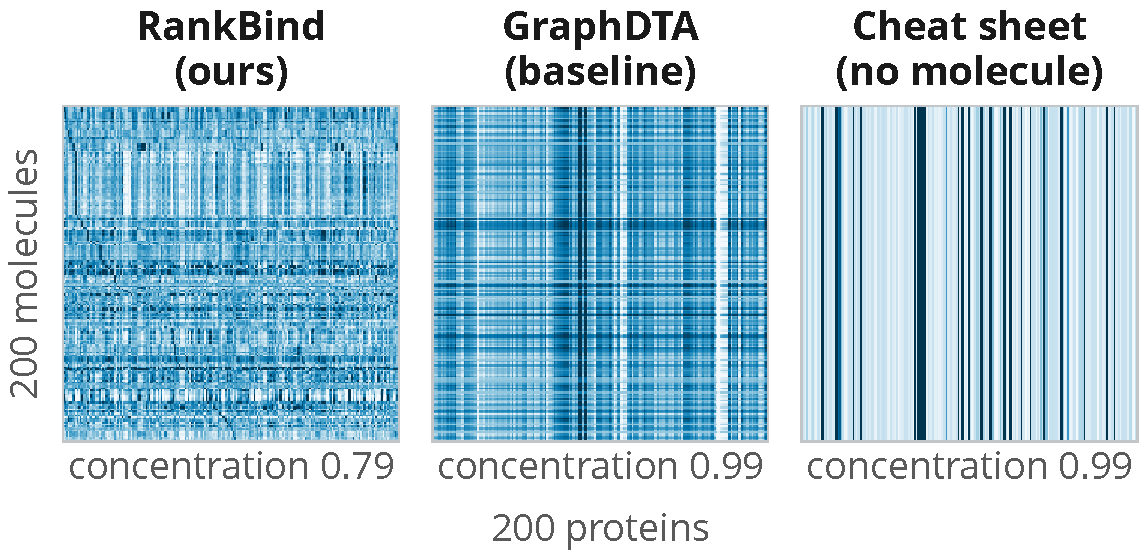
\includegraphics[width=\linewidth]{fig_respmaps.pdf}
  \caption{Score response maps on the $200 \times 200$ test pool (rows:
  molecules, columns: proteins, darker = higher score). A vertical stripe is
  a protein that wins almost every molecule. GraphDTA's map is the
  molecule-blind prior's; \method's is de-striped.}
  \label{fig:respmaps}
\end{figure}

The dissociation is not an artefact of our ranking metric. The per-molecule
AUC that prior work reports on test pairs rests on $n=4$ here (only four
test molecules have both a positive and a negative pair) and cannot support
a conclusion on its own. Evaluating the same metric on the full
$200\times200$ matrix (a column counts as positive iff it is a held-out test
positive; every other column is a negative) recovers $n=30$ and confirms the
reading: all four baselines sit between $0.43$ and $0.53$, i.e.\ at chance
(Tab.~\ref{tab:phase1}). We therefore use \mrr{} and Hit@$K$ on the same
matrix as the primary metrics; both are well-defined for every test
molecule. \mrr{} is the mean reciprocal rank of the true target within a
molecule's row: 1.0 would mean the true target always ranks first, and
uniform random ranking over 200 candidates gives $\approx 0.029$.

Gini deserves a verdict of its own, because it misled us at the start. We
conjectured, following discussions of ``attractor bias'' in DTI score
matrices, that a Gini near 1 would reveal a learned pathology. It does not:
a molecule-blind baseline produces the same value from the label marginal
alone. Gini is a dataset-geometry artefact on this corpus. We report it as a
descriptor and do not use it as a success metric.

\subsection{\method: four ingredients that enforce within-molecule ranking}
\label{sec:method}

\method{} freezes both encoders, ChemBERTa (384-d) for the molecule
\citep{chithrananda2020chemberta} and ESM2-650M (1280-d) for the protein
\citep{lin2023esm2}, and trains only two 256-d projectors and a low-rank
bilinear head
($s(L,P) = f(L)^\top (UV^\top + \mathrm{diag}(d))\, g(P) + b$, rank 128;
65{,}793 head parameters). Total trainable budget: 627{,}201. The four
ingredients that shape training are:

\begin{enumerate}[leftmargin=*,itemsep=1pt,topsep=2pt]
  \item \textbf{Within-ligand margin loss.} For each anchor $(L, P^+)$ and
        $k=4$ sampled negatives,
        $\mathcal{L} = \max(0,\ m - s(L,P^+) + s(L,P^-_i))$ with $m=1.0$.
        The loss compares scores \emph{inside one molecule's candidate
        set}, which is exactly what \mrr{} measures.
  \item \textbf{Online hard-negative mining.} At each epoch start the model
        re-scores the (positive-molecule $\times$ train-protein) matrix and
        draws the $k$ negatives from the 50 highest-scoring non-substrate
        proteins per anchor, instead of uniformly at random.
  \item \textbf{Protein-balanced sampling.} Each epoch draws a near-equal
        number of positive and negative pairs \emph{per protein}, so
        frequent proteins cannot dominate batches and re-imprint their
        prior.
  \item \textbf{Low-rank bilinear head} instead of an MLP-concat head at
        identical capacity.
\end{enumerate}

\begin{table}[t]
\centering
\caption{Three-seed means $\pm$ s.d.\ on BRENDA-200 under the pinned-split
protocol (every seed trains and evaluates on the canonical protein split),
ordered by \mrr{}.
The top row is a matched-capacity BCE control with the same encoders and
split. Removing the margin loss collapses \mrr{} by $11\times$ and pooled
AUC rebounds to $0.91$: the shortcut returns. Removing the balanced sampler
costs $33\%$. The MLP row is the matched-capacity control. A ten-seed
extension of the two head configs (run to test the reliability reading of
the three-seed spread gap) shows overlapping distributions --- bilinear
$0.182\pm0.075$ versus MLP $0.143\pm0.097$ --- so the head choice moves the
mean, not reliability. The last row re-selects checkpoints by
validation matrix \mrr{} instead of validation pooled AUC (selection-rule
sensitivity check). $^*$: the residue-attention row is a single-seed
mechanistic variant (Section~\ref{sec:residue}), not part of any multi-seed
comparison.}
\label{tab:ablation}
\small
\setlength{\tabcolsep}{4pt}
\begin{tabular}{lccccc}
\toprule
Config & \mrr{} & Hit@10 & Pooled AUC & Gini-res. & Top-10 \\
       &        &        &            &           & overlap \\
\midrule
BCE control (MLP head)        & 0.014$\pm$0.002 & 0.000$\pm$0.000 & 0.918$\pm$0.003 & $-0.003$ & 0.674$\pm$0.140 \\
$-$ margin loss               & 0.020$\pm$0.006 & 0.029$\pm$0.029 & 0.914$\pm$0.004 & $-0.058$ & 0.018$\pm$0.030 \\
$-$ balanced sampler          & 0.147$\pm$0.070 & 0.441$\pm$0.153 & 0.611$\pm$0.016 & $-0.068$ & 0.000$\pm$0.000 \\
$-$ bilinear head (MLP)       & 0.140$\pm$0.087 & 0.373$\pm$0.170 & 0.634$\pm$0.067 & $-0.149$ & 0.222$\pm$0.385 \\
\textbf{\method}              & \textbf{0.220$\pm$0.026} & 0.598$\pm$0.045 & 0.618$\pm$0.005 & $-0.197$ & 0.018$\pm$0.030 \\
$+$ matrix-MRR selection      & 0.183$\pm$0.055 & 0.539$\pm$0.103 & 0.584$\pm$0.035 & $-0.176$ & 0.092$\pm$0.034 \\
$+$ residue attention pool$^*$ & \textbf{0.316} & 0.706 & 0.646 & $-0.245$ & 0.000 \\
\bottomrule
\end{tabular}
\end{table}

Table~\ref{tab:ablation} orders the ingredients by what they buy. The margin
loss is the dominant contribution: without it \mrr{} falls from $0.220$ to
$0.020$ and pooled AUC jumps back to $0.91$ while the top-ten overlap with
the prior stays at $0.02$ --- the rebound rides the molecule-side shortcut
of Section~\ref{sec:shortcut}, not the protein marginal. The balanced sampler is a secondary positive
($-33\%$ when removed). The bilinear head wins on the mean ($0.220$
versus $0.140$, overlapping three-seed ranges). Extending both head configs
to ten seeds --- run precisely to test whether that gap reflects a
reliability advantage --- dissolves the stability reading: \mrr{}
$0.182\pm0.075$ for bilinear versus $0.143\pm0.097$ for MLP, a seed-spread
ratio of only $1.3\times$. We therefore claim no stability advantage; we
keep the bilinear form for the invariance of its interaction function
(Section~\ref{sec:simplearch}) and its higher mean.
Hard-negative mining, which is part of the
default rather than an ablation, lifts \mrr{} from $0.201$ to $0.247$ on the
shared seed-42 anchor ($+23\%$; single-seed comparison).

Two protocol checks confirm the headline is not an artefact of choices made
during training. First, checkpoint selection: the default selects the epoch
by validation pooled AUC --- the very metric this paper criticises. Re-running
all three seeds with selection on validation matrix \mrr{} instead (last row)
gives $0.183 \pm 0.055$, with a range overlapping the default's: the ranking
result does not switch on the selection rule. The variant is also
handicapped by design --- only two positive molecules fall in the
validation split, so matrix-\mrr{} selection there is effectively selection
on noise, which is why we keep pooled-AUC selection as the default and
report both. Second,
an earlier three-seed sweep had coupled the data split to the training seed,
and its evaluation silently rebuilt only the canonical split, so the
seed-7/1337 runs were scored largely on their own training pairs; every
multiseed number in this paper comes from the corrected pinned-split protocol
described in Section~\ref{sec:seeds}.

The BCE control row deserves emphasis: with the same encoders, the same
data and the same split, ordinary pair-wise BCE reproduces the published
baselines' pathology in full: pooled AUC $0.918$, \mrr{} $0.014$, top-ten
overlap with the molecule-blind prior $0.674$. The shortcut behaviour is
produced by the training recipe, not by the encoders or the data. A BCE
auxiliary loss added to the margin objective (weight 0.5) lifts pooled AUC
by only $+0.03$ ($0.623 \to 0.655$), nowhere near $0.80$: the high pooled
value is not a loss-function artefact that tuning could recover, it is the
shortcut itself.

Figure~\ref{fig:ablation} shows the same numbers as bars with seed error
bars; Fig.~\ref{fig:jaccard} measures shortcut avoidance directly as the
top-ten overlap of each model with the molecule-blind prior.

\begin{figure}[t]
  \centering
  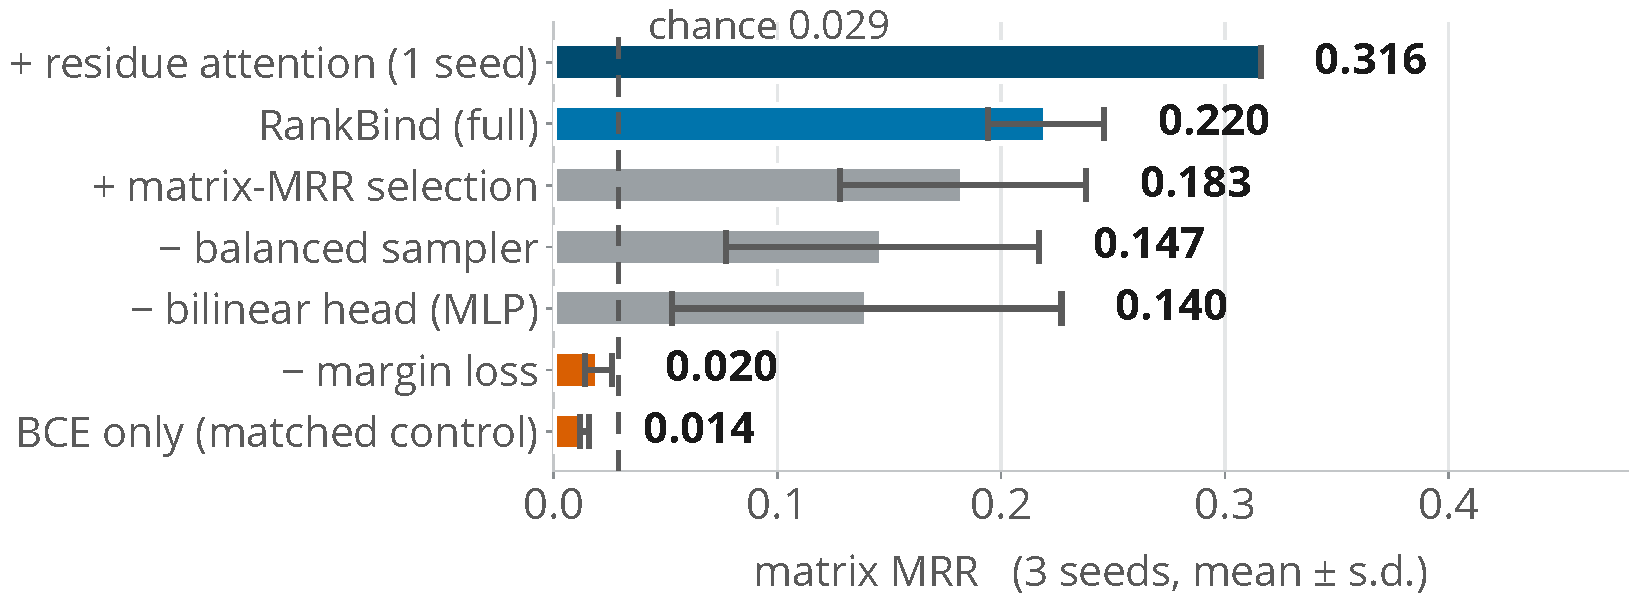
\includegraphics[width=0.75\linewidth]{fig_ablation.pdf}
  \caption{Ablation, three seeds, \mrr{} (chance 0.029 dashed). The BCE
  control (top bar) reproduces the published models' pathology inside our
  own codebase: the behaviour comes from the recipe, not the data.}
  \label{fig:ablation}
\end{figure}

\begin{figure}[t]
  \centering
  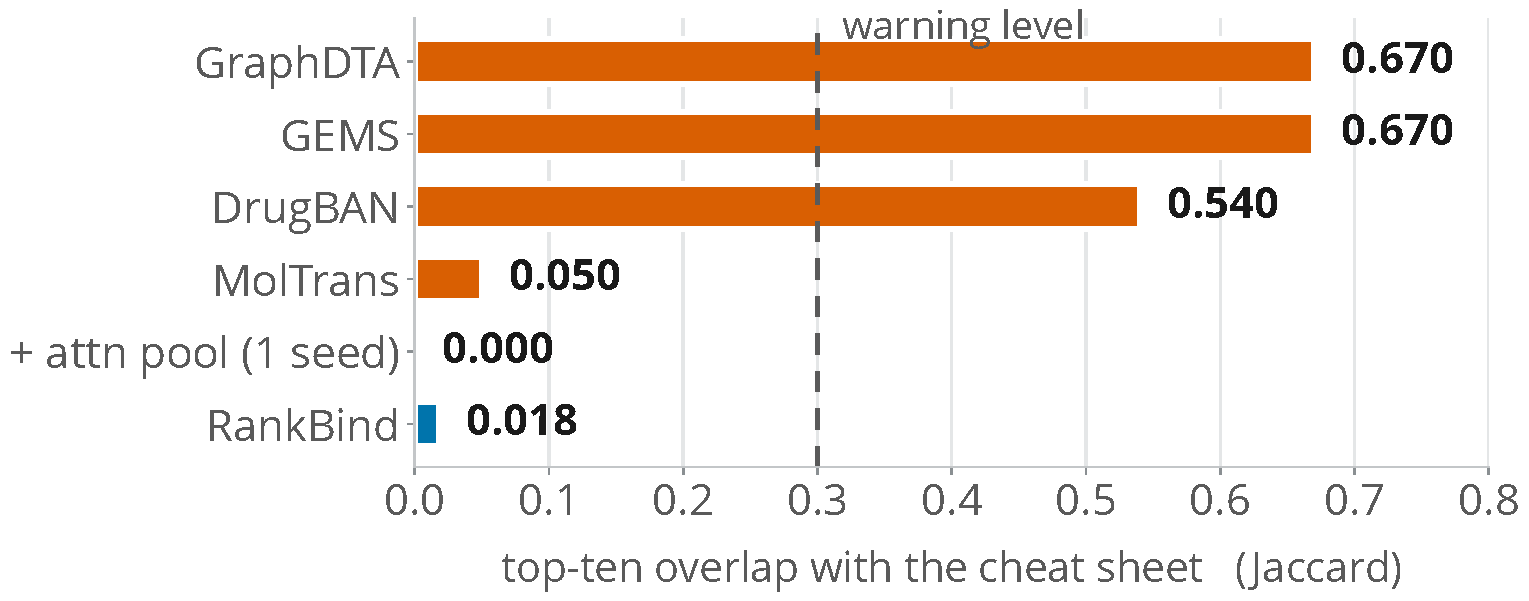
\includegraphics[width=0.75\linewidth]{fig_jaccard.pdf}
  \caption{Shortcut avoidance, measured directly: overlap of each model's
  ten favourite proteins with the molecule-blind prior's. The three
  baselines with a Jaccard of $0.54$--$0.67$ share two thirds of their
  favourites with a model that never sees the molecule.}
  \label{fig:jaccard}
\end{figure}

\subsection{A residue-level attention pool: small gain, and the audit says why}
\label{sec:residue}

This section is a \emph{single-seed mechanistic analysis}: the variant is
not replicated across seeds, it is not part of any headline comparison, and
its value here is what the audit reveals about protein encoding, not the
performance delta.

The default mean-pools the per-residue ESM2 tensor. We replace the mean pool
with a learned-query attention pool
($\alpha_i = \mathrm{softmax}(\mathbf{q}^\top \mathrm{LN}(\mathbf{e}_i)/\sqrt{d})$)
over the per-residue embeddings, adding 3{,}840 parameters ($+0.6\%$). On
the shared seed-42 anchor the variant reaches \mrr{} $0.316$ (from $0.247$),
Hit@10 $0.706$, per-molecule AUC $0.930$ --- a single-seed observation
($^*$ in Table~\ref{tab:ablation}), not yet replicated across seeds under
the pinned-split protocol.

\begin{figure}[t]
  \centering
  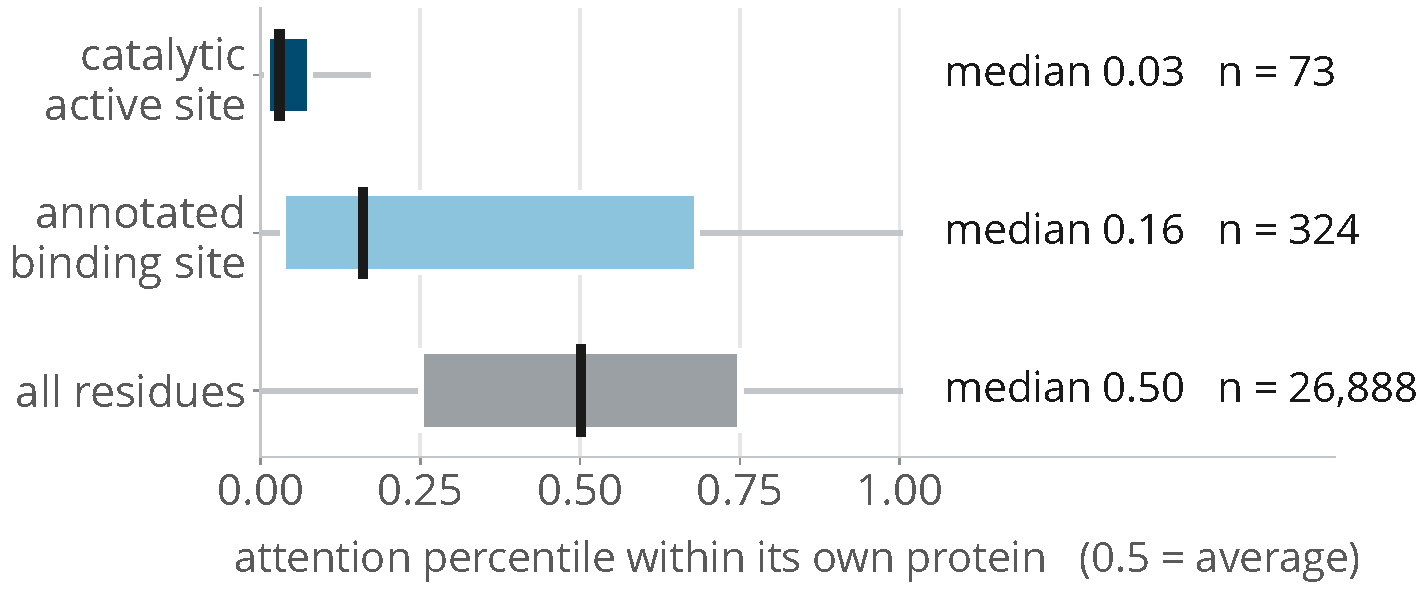
\includegraphics[width=0.8\linewidth]{fig_attention.pdf}
  \caption{Attention percentile of functional residues within their own
  protein (median over annotated residues; 0.5 = average). Catalytic
  active-site residues sit at the 3rd percentile: the pool de-weights the
  functional pocket instead of selecting it.}
  \label{fig:attention}
\end{figure}

Two audits explain what the pool actually does. First, the weights are
near-uniform: the median top-10\% mass is $0.118$ against a uniform
expectation of $0.10$, and the entropy sits at the ceiling $\log L$. The
pooled representation is therefore close to the mean of the
\emph{normalised} residue vectors (which is provably different from the v4
mean of the raw vectors, because per-residue LayerNorm rescales the
high-norm residues that dominate the raw mean). Second, the small residual
selection is reproducible across seeds (median Spearman $0.86$, random
expectation $\approx 0$) but it does not find the pocket: active-site
residues, annotated from UniProt, rank at the median 3rd attention
percentile of their own protein, and attention weights separate annotated
from unannotated residues with ROC-AUC $0.21$ (chance $0.5$; Fig.~\ref{fig:attention}).
What the reproducible rank order tracks is hydrophobicity: the within-protein
Spearman between attention and Kyte--Doolittle hydropathy is $+0.25$ with
the same sign in $58/60$ proteins.

The mechanism is therefore per-residue normalisation before pooling, not
learned pocket selection. This is a finding about residue-level encoding
worth stating plainly: raw mean-pooling lets a few high-norm residues
dominate the protein vector, and removing that artefact is what buys the
$+0.10$ \mrr{}. We report the attention pool because it is the module we
trained; a parameter-free LayerNorm-then-mean pool is the cheap variant that
should be tried first.

\subsection{Cold-ligand and double-cold splits: the dissociation does not need recurring molecules}
\label{sec:cold}

The canonical split holds out proteins but not molecules: 53.6\% of test-pair
ligands occur in training rows (Section~\ref{sec:shortcut}), which is what
makes ligand-level memorisation available as a shortcut ingredient. To test
whether this recurrence is \emph{required} for the pooled-AUC/ranking
dissociation, we rebuild BRENDA-200 twice with everything else held fixed ---
encoders, capacity class, training budget, hard-negative logic, evaluation
pool construction, seeds --- so that only the split definition changes. In
the \emph{cold-ligand} split, canonical molecule identities (canonical
SMILES, the same molecule definition used throughout the leakage audit) are
partitioned $70/15/15$ at seed 42: no test molecule has a training row,
while proteins recur as before ($94.5\%$ of test-pair proteins seen in
training). In the \emph{double-cold} split the two partitions are combined,
holding out molecules \emph{and} proteins simultaneously; pairs whose axes
land in different folds are dropped ($46\%$ of rows), leaving 213 test
pairs. Both splits verify $0.0\%$ test-molecule recurrence against $53.6\%$
for the canonical split, and every run manifest pins the realised overlap
fractions of both axes; evaluation refuses to run against a mismatched
split (Section~\ref{sec:seeds}).

The null baselines behave exactly as the split geometry dictates, and their
behaviour is itself informative (Tab.~\ref{tab:cold}). Under cold-ligand
the per-ligand rate prior collapses from $0.915$ to exactly $0.500$ ---
no test molecule has training rows --- while the molecule-blind protein
prior, capped at $0.500$ on the canonical split, now carries signal
($0.655$) because proteins recur: a mirror image of Table~\ref{tab:sources}.
Under double-cold both priors sit at exactly $0.500$: neither marginal
contains any information about test labels, so anything a model achieves
beyond them there cannot come from memorised marginals.

\begin{table}[t]
\centering
\caption{Stress-test splits of BRENDA-200 with everything except the split
definition held fixed: same frozen encoders, capacity class, optimiser,
training budget, hard-negative logic and pool construction as
Tables~\ref{tab:phase1}--\ref{tab:ablation}; three seeds per configuration
(cold-ligand), five for double-cold ($\{11, 202\}$ added because the seed
spread is widest there). Pooled AUC is computed over each split's full test
set; \mrr{} on the matched evaluation pool, chance $\approx 0.029$
(---: degenerate under the tie rule for constant or discrete scorers,
Methods). The double-cold pool contains six matched positive pairs, so its
matrix metrics are indicative rather than precise; its full-split columns
are primary. The canonical column repeats
Tables~\ref{tab:phase1}--\ref{tab:ablation} for orientation. Regenerable
from \texttt{null\_baseline\_firstclass\_*.csv} and
\texttt{cold\_split\_multiseed.csv}.}
\label{tab:cold}
\footnotesize
\setlength{\tabcolsep}{3.5pt}
\begin{tabular}{l rr rr rr}
\toprule
& \multicolumn{2}{c}{Cold-ligand} & \multicolumn{2}{c}{Double-cold} &
  \multicolumn{2}{c}{Canonical} \\
\cmidrule(lr){2-3}\cmidrule(lr){4-5}\cmidrule(lr){6-7}
Source & Pooled AUC & \mrr{} & Pooled AUC & \mrr{} & Pooled AUC & \mrr{} \\
\midrule
Random baseline         & 0.496           & --- & 0.535           & --- & 0.500           & --- \\
\nullprior              & 0.655           & --- & 0.500           & --- & 0.500           & --- \\
Per-ligand rate prior   & 0.500           & --- & 0.500           & --- & 0.915           & --- \\
\midrule
BCE control             & 0.850$\pm$0.018 & 0.028$\pm$0.013 & 0.813$\pm$0.010 & 0.025$\pm$0.006 & 0.918$\pm$0.003 & 0.014$\pm$0.002 \\
\textbf{\method}        & 0.591$\pm$0.041 & \textbf{0.295$\pm$0.064} & 0.573$\pm$0.051 & \textbf{0.092$\pm$0.078} & 0.618$\pm$0.005 & \textbf{0.220$\pm$0.026} \\
\bottomrule
\end{tabular}
\end{table}

The logic of the three splits is straightforward. On the canonical split a
sceptic could attribute the pooled-AUC inflation to memorisation of
recurring ligand identities. Under cold-ligand this channel is closed ---
no test molecule has a training row --- yet the BCE control still posts
pooled AUC $0.850 \pm 0.018$ at chance-level ranking (\mrr{} $0.028 \pm
0.013$; Hit@10 $0.04$): ligand recurrence alone cannot explain the
dissociation. Under double-cold, neither test molecules nor test proteins
recur and both molecule-blind marginals sit at exactly $0.500$, yet the
control still posts pooled AUC $0.813 \pm 0.010$ at chance-level ranking
(\mrr{} $0.025 \pm 0.006$; Hit@10 $0.00$): the dissociation persists after
the obvious molecule- and protein-marginal explanations have been removed.
These results rule out simple ligand or protein marginal memorisation as
the sole explanation for the residual pooled separation; the remaining
source is not resolved by the present experiments.

The BCE control still passes pooled AUC on both stress splits while its
within-molecule ranking stays at chance against a reference of $0.029$.
This is the strongest form of the diagnosis: the pairwise objective posts
a pooled value far above every null while failing the task-aligned metric,
and it does so where the split geometry leaves no memorised marginal to
ride. What sustains the residual pooled signal is an open question;
plausible candidates are generalisable similarity structure between unseen
test entities and their training relatives, and global statistics of the
role-pure decoy construction. The diagnostic conclusion does not depend on
resolving it: pooled separation persists where memorisation cannot.

\method{} retains ranking signal on both stress splits, at reduced
magnitude, and we report the reduction plainly. Under cold-ligand (three
seeds) it reaches
\mrr{} $0.295 \pm 0.064$ (control $0.028$, chance $0.029$) and Hit@10
$0.565 \pm 0.008$. Under double-cold --- where $46\%$ of rows are dropped,
no identity recurs, and the pool surface shrinks to six positive pairs ---
its advantage narrows to \mrr{} $0.092 \pm 0.078$ across five seeds versus
the control's $0.025 \pm 0.006$, with Hit@10 $0.233 \pm 0.253$: still above
the control, but with overlapping ranges and the widest seed noise we
observe anywhere. Two readings follow. First, the dissociation is not an
artefact of ligand recurrence --- it survives that recurrence's removal.
Second, the ranking objective's advantage does not depend on recurring
identities either, though it weakens precisely where the training signal is
thinnest; whether it can be recovered under double-cold conditions (for
example by re-tuning negative mining for the smaller training set) is left
open. We keep the canonical protein-stratified split as the main benchmark
throughout the paper --- it is the setting in which published baselines were
evaluated --- and present the cold splits as stress tests of the
explanation, not replacement leaderboards; each split answers a different
question (target generalisation, molecule generalisation, or both), and the
diagnostic of Section~\ref{sec:recipe} applies to all of them.

\subsection{The diagnosis and the recipe transfer to seven datasets}
\label{sec:transfer}

Every dataset in this section is scored twice: with \method{} and with a
matched BCE control (same encoders, same split, ordinary pair-wise BCE),
because only a model trained on the same data can show what the standard
recipe buys there. Beyond three enzyme-wide datasets curated from the BRENDA
and SABIO-RK kinetics databases, each labelling enzyme--substrate pairs by a
measured kinetic quantity (catalytic efficiency kcat/$K_M$, Michaelis
constant $K_M$, turnover rate; 42--57k pairs, 3.8--9.5k proteins) we add
ESP,
an independent enzyme--substrate corpus \citep{kroll2023esp}, and three
kinase affinity benchmarks from the Therapeutics Data Commons
\citep{huang2021tdc}: BindingDB\textsubscript{$K_d$}, Davis
\citep{davis2011kinase} and KIBA \citep{tang2014kiba}, binarised at the
DeepDTA convention \citep{ozturk2018deepdta}. One caveat on provenance:
the decoys in the BRENDA-derived corpora are author-generated
(Section~4.1), so part of each pooled-AUC inflation is a property of this
benchmark design; the synthetic construction of Section~2.1, which uses no
decoys at all, carries the metric-side argument to settings where none are
injected. The transfer protocol differs from the BRENDA-200 headline
protocol in two documented ways: the BRENDA-200 headline values rest on
three seeds, whereas the transfer runs are single-seed (the seed-42
anchor; supplementary seeds for the three BRENDA+SABIO families exist and
are discussed in Section~3), and the hard-negative pool is scaled to the
training-protein count of each dataset (Section~4.3), because the
BRENDA-200-tuned pool of 50 is meaningless at 3.8--9.5k training proteins.
Each run's split, pool size and realised overlap fractions are pinned in
its manifest (Section~4.5), and every row of Table~\ref{tab:seven} is
regenerable from the committed aggregate tables. Each dataset is evaluated on
the same instruments as BRENDA-200: a matched 200-protein pool, \mrr{} and
Hit@K within each molecule, the molecule-blind prior as reference.

\begin{table}[t]
\centering
\caption{Seven datasets, each scored with a matched BCE control and
\method. The control passes pooled AUC on all seven datasets (0.84--0.98)
while ranking at near-chance \mrr{} (chance $\approx 0.029$): the BRENDA
dissociation is reproduced on every corpus tested. \method{} ranks $7$--$25\times$
better than the control on the catalytic enzyme datasets; on ESP it keeps
pooled AUC 0.891 while ranking best of all. The two kinase affinity sets
with no ranking signal in the prior (Davis, KIBA) bound the claim.
BRENDA+SABIO and ESP rows use pool sizes of roughly half the
train-protein count (Section~\ref{sec:transfer}; single seed);
Davis/KIBA/BindingDB use the default pool of 50.}
\label{tab:seven}
\footnotesize
\setlength{\tabcolsep}{3.5pt}
\begin{tabular}{llrrrrr}
\toprule
Dataset & Model & $n_{\text{pos}}$ & Pooled AUC & \mrr{} & $\rho_{\text{row}}$ vs.\ prior & Top-10 overlap \\
\midrule
\multicolumn{7}{l}{\emph{Enzyme--substrate}}\\
kcat/$K_M$ (BRENDA+SABIO) & BCE control & 76 & 0.948 & 0.029 & $+0.09$ & 0.053 \\
                          & \method     & 76 & 0.619 & \textbf{0.228} & $+0.01$ & 0.053 \\
$K_M$ (BRENDA+SABIO)      & BCE control & 59 & 0.978 & 0.030 & $+0.20$ & 0.111 \\
                          & \method     & 59 & 0.633 & \textbf{0.219} & $-0.04$ & 0.053 \\
turnover (BRENDA+SABIO)   & BCE control & 35 & 0.966 & 0.014 & $+0.10$ & 0.000 \\
                          & \method     & 35 & 0.603 & \textbf{0.344} & $-0.06$ & 0.111 \\
ESP                       & BCE control & 50 & 0.897 & 0.098 & $+0.01$ & 0.053 \\
                          & \method     & 50 & 0.891 & \textbf{0.387} & $-0.02$ & 0.000 \\
\midrule
\multicolumn{7}{l}{\emph{Kinase affinity (not enzyme--substrate)}}\\
BindingDB\textsubscript{$K_d$} & BCE control & 25 & 0.844 & 0.042 & $+0.48$ & 0.176 \\
                               & \method     & 25 & 0.692 & \textbf{0.320} & $+0.09$ & 0.053 \\
Davis                        & BCE control & 94 & 0.878 & 0.044 & $+0.42$ & 0.176 \\
                             & \method     & 94 & 0.682 & 0.038 & $+0.22$ & 0.000 \\
KIBA                         & BCE control & 453 & 0.856 & 0.035 & $+0.35$ & 0.111 \\
                             & \method     & 453 & 0.492 & 0.023 & $-0.15$ & 0.111 \\
\bottomrule
\end{tabular}
\end{table}

Four observations follow from Table~\ref{tab:seven}. First, the shortcut
precondition is not specific to BRENDA-200: the molecule-blind prior's
score distribution is as concentrated on every dataset tested here as on
BRENDA (Gini $\approx 0.995$), so the skewed per-protein label distribution
that enables the shortcut occurs across the tested corpora. Second, the BCE
control exploits it on every dataset tested: pooled AUC
$0.84$--$0.98$ at near-chance \mrr{} ($0.014$--$0.098$), exactly the
dissociation of Section~2.1, now on six corpora beyond BRENDA-200. Third,
\method\ circumvents it on each catalytic enzyme dataset tested: \mrr{} $0.228$,
$0.219$, $0.344$ against control values of $0.029$, $0.030$, $0.014$
($7$--$25\times$), with the per-row correlation to the prior between
$+0.01$ and $-0.06$, an order of magnitude below the control's $+0.09$
to $+0.20$. ESP, the one independent enzyme--substrate corpus, is the
instructive
exception: it carries genuine per-molecule signal (both models reach
per-molecule AUC around $0.85$ or above), and once the hard-negative pool is scaled to
its protein count \method{} ranks best of all seven datasets (\mrr{} $0.387$,
$4\times$ the control) while keeping pooled AUC at $0.891$. Where real
signal exists, no shortcut trade-off is needed.

Fourth, two honest non-wins bound the claim. On the kinase affinity sets the
molecule-blind prior carries no ranking signal at all (\mrr{} $0.016$--$0.021$,
at chance), so there is nothing to circumvent. BindingDB\textsubscript{$K_d$}
is the one affinity set where \method{} ranks well ($0.320$); Davis shows
low \mrr{} ($0.038$) but a healthy per-molecule AUC of $0.686$, a metric
artefact of promiscuous kinase inhibitors with many positive proteins per
molecule; on KIBA, \method's training did not converge to a ranking
solution (per-molecule AUC $0.457$), a tuning limitation on our side, not a
refutation of the diagnosis.

The BRENDA+SABIO rows also resolve a scaling question from our first
transfer run. With the BRENDA-200-tuned hard-negative pool of 50, \mrr{} on
these datasets was $0.134$, $0.023$ and $0.040$ (1.6--9.7 times
below the BRENDA-200 headline) while the correlation with the prior stayed
at zero. The drop looked like a loss of signal but was a coverage artefact:
a pool of 50 covers a quarter of BRENDA-200's training proteins but less
than 2\% of a 3.8--9.5k-protein training set, so hard-negative mining
degrades to random sampling. Scaling the pool to roughly half of the train
proteins (1{,}400, 3{,}400 and 2{,}000) lifts \mrr{} monotonically to the
values in the table, with the anti-shortcut property unchanged. The same
fix, a pool of 4{,}000, was applied to ESP.

\subsection{A five-point recipe}
\label{sec:recipe}

On the benchmarks studied here, the evidence reduces to five
recommendations. We recommend the checklist wherever ligand or protein
marginals may dominate pooled metrics --- enzyme--substrate corpora with
recurring molecules above all.

\begin{enumerate}[leftmargin=*,itemsep=2pt,topsep=2pt]
  \item \textbf{Run the molecule-blind null before reporting pooled
        metrics.} Score each pair by the protein's training positive rate.
        If your model matches this baseline in pooled AUC and overlaps it
        in the top-$K$ proteins (Jaccard $\geq 0.30$), pooled AUC certifies
        the prior, not ligand-conditional discrimination. The probe is one
        matrix multiply.
  \item \textbf{Optimise within-molecule ranking, not pair-wise
        classification.} A margin loss over negatives sampled inside each
        molecule's candidate set is the single largest lever in our
        ablation. Do not add BCE as an auxiliary: it recovers the pooled
        number without fixing the ranking.
  \item \textbf{Balance the sampler per protein.} Otherwise frequent
        proteins re-imprint their label prior into every batch.
  \item \textbf{Scale the hard-negative pool with the number of train
        proteins.} A pool tuned on a 200-protein benchmark is meaningless
        at 5{,}000 proteins. Half of the train-protein count worked
        everywhere we tried it.
  \item \textbf{Do not gate model selection on pooled AUC.} Report it for
        comparability, but gate on three-seed \mrr{}. The metric you gate
        on should not be the metric the shortcut inflates.
\end{enumerate}

%===============================================================================
\section{Discussion}
\label{sec:discussion}

The central observation of this paper is methodological: on the
enzyme--substrate benchmarks studied here, pooled AUC validates the wrong
property --- it can be high while ligand-conditional ranking sits at
chance. We do not claim this holds for every DTI benchmark; on the kinase
affinity sets (Davis, KIBA) the molecule-blind prior carries no ranking
signal at all (Section~2.5), so there is no shortcut of the kind diagnosed
here for pooled AUC to certify. Four published models,
one of them built on pretrained protein language models, all pass it, and
three of the four reproduce the per-protein label marginal in their score
structure (top-ten overlap $54$--$67\%$ with the molecule-blind prior;
MolTrans $5\%$). On this
split the protein marginal itself cannot be the source --- a molecule-blind
protein prior scores exactly $0.500$, chance, because no test protein has
training rows; what pooled AUC certifies here are molecule-level regularities
that the decoy protocol makes trivial to memorise (Section~2.1). The fix is
not a better encoder or a bigger
dataset; it is an evaluation change (rank inside each molecule) and a
training change (optimise that ranking directly). \method{} is the concrete
instance of the latter, and its ablation shows the mechanism: the margin
loss is what keeps the model honest, and the balanced sampler and
hard-negative mining support it. The bilinear head is kept for its
invariant interaction form, not because it trains more reliably
(Section~\ref{sec:method}).

The cost deserves to be stated plainly. On BRENDA-200, relative to the BCE
control, \method{} trades pooled AUC down from $0.92$ to $0.62$ while \mrr{}
goes from $0.014$ to $0.220$. We consider this the right trade: the high
pooled value was never valid, and the ranking value is what the task asks
for. ESP shows that the trade is not inherent to the recipe: there, real
per-molecule signal exists, and \method{} keeps pooled AUC at $0.891$ while
ranking best of all seven datasets.

Three limitations bound the claims. First, the transfer table reports the
seed-42 anchor per dataset; supplementary extra seeds under the pinned-split
protocol exist for the three BRENDA+SABIO families and show substantial
seed spread (matrix MRR ranges $0.199$--$0.280$ for kcat/$K_M$,
$0.166$--$0.219$ for $K_M$,
$0.242$--$0.344$ for turnover), so transfer point estimates carry roughly
$\pm 0.05$ seed noise; on BRENDA-200 itself, extending the two head configs
to ten seeds widens the full-model spread to $\pm 0.075$
(Section~\ref{sec:results}), so headline point estimates should be read as
$\pm 0.05$--$0.08$ rather than $\pm 0.03$. Second, the molecule-side
shortcut quantified in Section~2.1 (role-pure ligands, recurring
molecules, a ligand-only linear probe at $0.887$ pooled AUC) means
absolute pooled values on this corpus are bounded below by molecular
memorisation; \method{} sits at $0.618$, and the seven-dataset control
comparison is the cleaner instrument. Third, the residue-level
attention does not find catalytic pockets (it de-weights them), so any
future pocket-selection scheme should use structural priors (AlphaFold
structures plus a pocket detector) rather than learned attention.

What we hope survives this paper is the probe, not the architecture. Any
DTI model can be checked against the molecule-blind prior in minutes, and
any dataset can be scored with \mrr{} instead of pooled AUC alone. The
recipe of Section~\ref{sec:recipe} is the cheapest way we found to pass that check: 627k
trainable parameters, a few hours on one GPU per seed, and every ingredient
is a standard technique from metric learning.

%===============================================================================
\section{Methods}
\label{sec:methods}

\subsection{Data and splits}
\label{sec:data}

BRENDA-200 is the enzyme--substrate corpus used throughout
Sections~2.1--2.4: a $200\times200$ subset of the BRENDA+SABIO
enzyme--substrate records (hydrolytic enzymes dominate; 9{,}632 pairs, of
which 3{,}175 are documented substrates and 6{,}457 are decoys). Each
positive pair is a molecule recorded as a substrate of the enzyme in BRENDA
\citep{chang2021brenda} or SABIO-RK \citep{wittig2018sabiork}; the decoys
are non-substrate pairs (value 0) whose molecules are structurally similar
to the enzyme's true substrates (median Tanimoto similarity 0.48 to the
closest one), injected by the project's decoy pipeline. The protocol
assigns each molecule a fixed role: of the 4{,}604 unique ligands, 1{,}417
appear only as documented substrates and 3{,}157 only as decoy carriers
(99.3\% label-pure). The split is
protein-stratified (seed 42, $70/15/15$) so that test proteins never appear
in training; the test set holds 1404 pairs over 200 unique proteins and 200
unique molecules, and all matrix metrics are computed on this pool. The
split is implemented once in \texttt{baselines/adapters/common.py::
BRENDADataConfig.get\_protein\_split} and reused by every model and every
diagnostic.

Two stress-test variants of the same corpus hold out molecules as well
(Section~\ref{sec:cold}). Molecule identity is the canonical SMILES string
(\texttt{substrate\_smiles\_canon}), the same molecule definition used by
the leakage audit. The cold-ligand split partitions unique identities
$70/15/15$ at seed 42; the double-cold split intersects this partition with
the canonical protein split and drops pairs whose two axes land in different
folds ($46\%$ of rows). Both are implemented in
\texttt{BRENDADataConfig.get\_ligand\_split} /
\texttt{get\_double\_cold\_split}, selected by the configuration key
\texttt{data.split\_mode}, and every run manifest records the realised
train/test overlap fractions for both axes alongside the pair counts. The
evaluation guard of Section~\ref{sec:seeds} applies unchanged: it refuses to
score a model on a split other than the one it trained on.

The three enzyme-wide datasets are produced by the project's pinned data
pipeline (the \texttt{reactionDataFiltering} git submodule, fixed commit):
a raw BRENDA+SABIO export (snapshot of 2026-04-29) is filtered to one
kinetic parameter (catalytic efficiency kcat/$K_M$, Michaelis constant
$K_M$, or turnover rate) and EC class; decoys are generated with a
MolTransformer-based decoy generator in offline mode (seed 42); and the two
are augmented into the with-decoys tables used here (\texttt{kcat\_km}:
43k pairs / 3.8k proteins / 13.1k SMILES; \texttt{km}: 57k / 9.5k / 14.6k;
\texttt{turnover}: 42k / 5.7k / 13.5k). Every pipeline stage writes a
sidecar manifest with the SHA-256 of its inputs and outputs, its parameters
and tool versions, so every table can be traced back to the raw export.
ESP \citep{kroll2023esp}, obtained
from its authors' release and re-split protein-stratified; and the kinase
affinity sets Davis \citep{davis2011kinase}, KIBA \citep{tang2014kiba} and
BindingDB\textsubscript{$K_d$} from the Therapeutics Data Commons
\citep{huang2021tdc}, binarised at the DeepDTA convention
\citep{ozturk2018deepdta} (Davis/BindingDB $\text{p}K_d \geq 7$, KIBA score
$\geq 12.1$) and split cold-target (unseen test proteins). For each dataset
a 200-protein evaluation pool is matched so that the pool proteins overlap
the training set to a comparable degree across datasets (61--71\%).

\subsection{Null baselines and metrics}
\label{sec:metrics}

The molecule-blind prior \nullprior{} scores each pair $(L, P)$ with the
training positive rate of $P$; the random baseline scores uniformly. Gini is
computed on the attractor shares of the score matrix (the per-protein
fraction of molecules for which the protein is the top-scoring partner);
0.5 means the shares are uniform, 1.0 that one protein wins every molecule.
The \emph{Gini-residual} subtracts the prior's Gini from the model's:
zero means the model matches the label marginal's concentration, negative
values mean a more even spread of top ranks.
The top-ten overlap is the Jaccard index between a model's ten largest
attractor shares and the prior's. The per-row Spearman $\rho$ correlates,
within each molecule's row,
the model's scores with the prior's; values at or below zero mean the model
does not ride the protein marginal.

\mrr{} is the mean reciprocal rank of the true target protein within each
test molecule's row of the $200\times200$ matrix (chance $\approx 0.029$
at 200 candidates); Hit@$K$ is the fraction of test molecules whose true
target lands in the top-$K$. Averaging is pair-weighted: every positive
(molecule, protein) pair contributes one reciprocal rank, so molecules with
several documented substrates weigh proportionally; the molecule-level
paired bootstrap of Section~\ref{sec:intro} instead averages one value per
test molecule, with test positives re-derived from the pinned split.
Ranks count strictly higher-scoring columns,
so ties are resolved optimistically; trained models' continuous scores make
this immaterial, but a constant scorer would receive \mrr{} $=1$, which is
why the prior's ranking metrics are excluded from comparison.
Per-molecule AUC is computed per row and
averaged; the test-pair variant rests on $n=4$ on BRENDA-200, the matrix
variant on $n=30$ (a column is positive iff it is a held-out test positive,
all other columns are negative). Pooled AUC and AUPR are reported for
comparability with prior work but are not used as success gates.

\subsection{Model and training}
\label{sec:model}

Molecules are embedded with frozen ChemBERTa, a language model pretrained
on molecular SMILES strings (384-d mean pool)
\citep{chithrananda2020chemberta}, proteins with frozen ESM2-650M, a
protein language model pretrained on 65M sequences (1280-d; mean pool in the
default, learned-query attention pool in the residue-level
variant) \citep{lin2023esm2}. Two-layer projectors map both to 256-d; the
score is computed by a low-rank bilinear head with diagonal correction and
bias (rank 128). Total trainable parameters: 627{,}201.

\subsubsection{A deliberately simple diagnostic architecture}
\label{sec:simplearch}

We intentionally avoid introducing a novel encoder architecture. Conceptually,
$\mathbf{z}_L = f_{\mathrm{lig}}(L)$ and $\mathbf{z}_P =
f_{\mathrm{prot}}(P)$ are frozen-encoder features passed through two-layer
projectors, and the score is $s(L,P) = \mathbf{z}_L^\top \mathbf{W}
\mathbf{z}_P + \mathbf{d}^\top(\mathbf{z}_L \odot \mathbf{z}_P) + b$ with
low-rank $\mathbf{W}$ and diagonal correction $\mathbf{d}$. The bilinear
form gives an explicit cross-modal interaction at low parameter cost and
constructs the full score matrix directly, which is what our evaluation
requires. Neither the encoder components nor the interaction function are
presented as innovations: \method\ is a controlled experimental vehicle for
testing whether ligand-conditional ranking reduces shortcut behaviour, not
an architectural proposal. The design makes the causal comparison clean ---
the BCE control of Section~2.2 uses identical encoders, split and capacity,
so any difference in ranking behaviour is attributable to the objective,
sampling and negative mining rather than to architectural capacity.

Training uses AdamW ($\mathrm{lr} = 3\times10^{-4}$, cosine decay to
$3\times10^{-5}$, weight decay $10^{-4}$, gradient clipping at 1.0), bf16,
batch size 32 molecules, up to 50 epochs, early stopping on validation
pooled AUC with patience 10 (minimum 20 epochs; the selection-rule
sensitivity variant of Section~2.2 replaces this criterion with validation
matrix \mrr{}). The balanced sampler draws
16 pairs per protein per epoch with a 1:1 positive:negative ratio. The
hard-negative pool is 50 on BRENDA-200 and the affinity benchmarks, and
scaled to $\approx 50\%$ of the training protein count on the enzyme-wide
datasets (1{,}400 / 3{,}400 / 2{,}000 / 4{,}000 for kcat/$K_M$, $K_M$,
turnover, ESP). The BCE control uses the same encoders and split with a
binary cross-entropy loss, random batches and the MLP-concat head. The BCE
auxiliary probe adds a BCE term of weight 0.5 to the margin objective.

Seeds $\{42, 7, 1337\}$ are used for all BRENDA-200 configurations
(Sections~2.1--2.4), including the cold-split stress tests of
Section~\ref{sec:cold}; the double-cold configurations are additionally
extended to five seeds ($\{11, 202\}$ added, because their seed spread is
the widest we observe). The transfer runs of Section~\ref{sec:transfer}
report the seed-42 anchor in Table~3, with supplementary extra seeds (7 and
1337) for the three BRENDA+SABIO families. Hardware: one NVIDIA A30 GPU per run, about 1.5\,h per seed for the
default and 4\,h for the residue-level variant.

\subsubsection{Seeds and split pinning}
\label{sec:seeds}

The protein-stratified train/val/test split is drawn once with a dedicated
random seed (42) that is independent of the training seed; training seeds
$\{42, 7, 1337\}$ vary only weight initialisation, batch shuffling and
negative sampling. For the head comparison of Section~2.3 both the bilinear
and MLP configurations were additionally extended to ten seeds
($\{1, 2, 3, 5, 6, 8, 11\}$ added); all other rows keep the registered
three-seed protocol, and Table~2 reports matched three-seed values for
comparability across rows. Evaluation rebuilds the split from the recorded
configuration and refuses to run if it does not match the one stored in a
run's manifest, which rules out scoring a model on pairs it trained on ---
an error mode we caught in an internal audit of an earlier sweep and
corrected before aggregating any of the numbers reported here.

\subsection{Attention audit}
\label{sec:audit}

Attention weights were inspected for three seeds and 60 sampled BRENDA
proteins. Cross-seed agreement is the median Spearman correlation of the
weight vectors between seed pairs (random expectation $\approx 0$).
Functional residues were annotated from UniProt records (active sites,
binding sites, signal peptides) \citep{uniprot2023}; the attention
percentile of a residue is its rank within its own protein. Within-protein
correlations with per-residue descriptors (Kyte--Doolittle hydropathy
\citep{kytedoolittle1982}, Chou--Fasman propensities
\citep{choufasman1978}, net charge, ESM2 residue norm) were computed per
protein and aggregated by the sign-consistency across proteins.

\subsection{Provenance}
\label{sec:provenance}

Every training run writes a \texttt{manifest.json} pinning the resolved
configuration, git commit, library versions, input-data SHA-256 and the
SHA-256 of the best checkpoint and score matrix. The three-seed means in
Tables~\ref{tab:phase1}--\ref{tab:ablation} are aggregated by
\texttt{scripts/aggregate\_multiseed.py}, the stress-split table by
\texttt{scripts/aggregate\_cold\_splits.py}, all from these manifests. All code,
configurations and the aggregated result tables are public at
\url{https://github.com/christophmanitz/rankbind} (paper: \texttt{paper/}).
The per-run manifests and score matrices that pin the reported numbers are
archived with the HPC runs that produced them; \texttt{REPRODUCIBILITY.md}
lists every artefact and the command that regenerates it.

%===============================================================================
\section*{Data availability}
All source code, configurations and the scripts that regenerate every table
and figure are available at \url{https://github.com/christophmanitz/rankbind};
the aggregated result tables are committed alongside the code. The input
data (the processed BRENDA-200 split with decoys, a few MB) and the
per-run artefacts (manifests, score matrices, checkpoints) are not
redistributed in the repository; \texttt{REPRODUCIBILITY.md} lists each
artefact, its SHA-256 and the command that regenerates it, and the
artefacts are available from the authors on request. The enzyme-wide
datasets are derived from the public BRENDA~\citep{chang2021brenda} and
SABIO-RK~\citep{wittig2018sabiork} resources (derivation pipeline pinned as
a git submodule), and the external benchmarks are obtained from their
original sources via the Therapeutics Data Commons~\citep{huang2021tdc}.

\section*{Code availability}
Training, evaluation and null-probe code lives in the \texttt{v5\_rankbind/}
and \texttt{evaluation/} directories of the repository; the reproduction
commands are listed in \texttt{REPRODUCIBILITY.md}.

%===============================================================================
\bibliographystyle{plainnat}
\bibliography{references}

\end{document}